Two main experiments were conducted in order to test the implemented Naive Bayes classifier. Both of them gave poor results in terms of accuracy. This is due to the small size of the dataset. Only 14 examples of a dataset with 4 categorical predictors isn't enough to properly train the classifier. Taking into account that number of levels for each predictor, there are 72 possible level-predictor-class combinations of which we only have 14, leaving room for uncertainty.

\begin{table}[]
	% increase table row spacing, adjust to taste
	\renewcommand{\arraystretch}{1.3}
	% if using array.sty, it might be a good idea to tweak the value of
	% \extrarowheight as needed to properly center the text within the cells
	\caption{Misclassified observations (red = highly misclassified, yellow = moderately misclassified, light yellow = rarely misclassified)}
	\label{tbl:misclassifications}
	\centering
	% Some packages, such as MDW tools, offer better commands for making tables
	% than the plain LaTeX2e tabular which is used here.
	\begin{tabular}{|>{\em}c|c|c|c|c||c|}
		\hline
		index & Outlook  & Temperature & Humidity & Windy & Play \\ \hline \hline
		\rowcolor{Yellow}
		1 & overcast &  hot        &  high    &  FALSE & yes \\ \hline
		  & overcast &  cool       &  normal  &  TRUE  & yes \\ \hline
		\rowcolor{Yellow}
		2 & overcast &  mild       &  high    &  TRUE  & yes \\ \hline
		  & overcast &  hot        &  normal  &  FALSE & yes \\ \hline
		\rowcolor{lightYellow}
		3 & rainy    &  mild       &  high    &  FALSE & yes \\ \hline
		\rowcolor{Yellow}
		4 & rainy    &  cool       &  normal  &  FALSE & yes \\ \hline
		\rowcolor{Red}
		5 & rainy    &  cool       &  normal  &  TRUE  & no \\ \hline
		\rowcolor{Yellow}
		6 & rainy    &  mild       &  normal  &  FALSE & yes \\ \hline
		\rowcolor{lightYellow}
		7 & rainy    &  mild       &  high    &  TRUE  & no \\ \hline
		\rowcolor{lightYellow}
		8 & sunny    &  hot        &  high    &  FALSE & no \\ \hline
		  & sunny    &  hot        &  high    &  TRUE  & no \\ \hline
		\rowcolor{lightYellow}
		9 & sunny    &  mild       &  high    &  FALSE & no \\ \hline
		\rowcolor{Yellow}
		10& sunny    &  cool       &  normal  &  FALSE & yes \\ \hline
		\rowcolor{Red}
		11& sunny    &  mild       &  normal  &  TRUE  & yes \\ \hline
	\end{tabular}
\end{table}
\begin{figure}
	\centering
	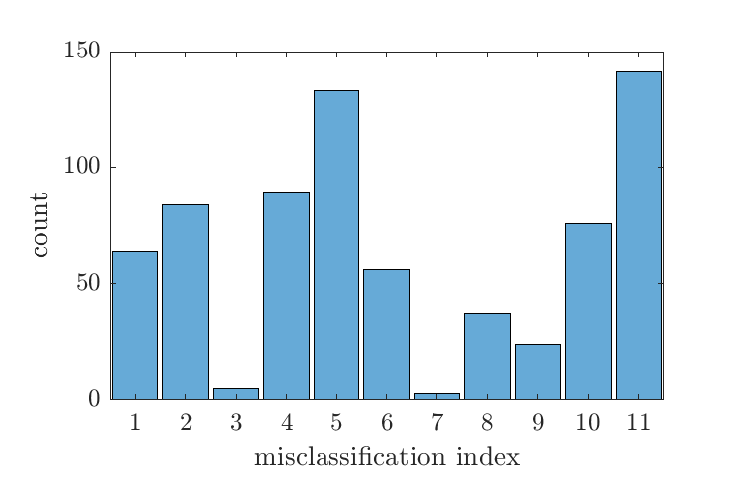
\includegraphics[width=0.4\textwidth]{misclassifications.eps}
	\caption{Misclassification histogram}
	\label{fig:misclassifications}
\end{figure}

Another common practice is to look for outliers or observations frequently misclassified. An analysis on these shows that, when running with 500 iterations, 11 out of the total 14 observations get misclassified at least once. Table \ref{tbl:misclassifications} and figure \ref{fig:misclassifications} complement each other to show which observations get the most misclassified. It is hard to explain exactly why they get misclassified since we're using stratified random splitting; however, misclassification may be caused by a high correlation of features in some training splits, leading to over inflating importance.